\documentclass[a4paper,12pt]{report}
\usepackage{fullpage}
\usepackage{hyperref}
\usepackage{graphicx}
\usepackage[backend=biber]{biblatex}
\addbibresource{/home/ramprakash/.dotfiles/bib/datacompr.bib}
\addbibresource{/home/ramprakash/.dotfiles/bib/wavelets.bib}

\title{A Study \& Implementation of the Embedded Zerotree Wavelet Algorithm \\ Proposal Report}
\author{
    C. Ramprakash (4NI18EC019) \\ Skanda Prasad (4NI18EC085)
    \\
    \\
    \hline
    \\
    Under the guidance of Dr. Raghu J. Mandya \& Dr. Narasimha Kaulgud
    \\
    Department of ECE
    \\
    The National Institute of Engineering, Mysuru
}
\date{May 2021}

\begin{document}

\maketitle

\tableofcontents

\chapter{Introduction}
\section{Overview}
The project aims to implement the \textbf{Embedded Zerotree Wavelet} algorithm
as a C library. It employs the well known \textit{Discrete Wavelet Transform}
as a tool for compression. The algorithm will be studied under several
operating conditions and demands, such as varying levels of
compression,``bit-budget'', etc

\section{The transform coder}

\begin{figure}[h]
    \centering
    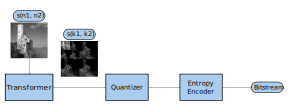
\includegraphics[scale=0.5]{../img/block-diag_shrunk.pdf}
    \caption{Transform coder: Generalised \cite{shap1993}}
    \label{fig:tcoder}
\end{figure}

A step-wise approach towards implementing this algorithm is taken, wherein
the each step is represented by a block in figure \ref{fig:tcoder}.

\pagebreak

\subsection{The transformer}
The transformer performs a mathematical transform on the supplied image. The
transform must satisfy 2 key properties, namely:
\begin{itemize}
    \item Full invertibility
    \item Separability
\end{itemize}

A few transforms that satisfy these conditions are the Fourier transform, the
discrete cosine transform and the wavelet transform. We will be using the
wavelet transform, since it is very handy when it comes to multi-resolution
analysis.

\subsection{The quantizer}

\subsection{The entropy encoder}

\chapter{Literature Survey}
The EZW algorithm generates a transformed and compressed bit-stream (embedded
coding) which is just enough to distinguish the compressed image with a null
image \cite{shap1993}. It ensures that the "important" bits are embedded at the
beginning of bit-stream i.e. low-frequency sub-bands contain the bulk of the
information. The sole purpose of this technique is to provide a reasonable
amount of image information for recovery after compression, at lower magnitudes
of bit-budget.

\par

EZW accomplishes this task by applying the \textit{Discrete Wavelet Transform}
on the individual rows and column of the digital image and in turn, dividing
the samples into various frequency sub-bands (LL, HL, LH, HH) in a hierarchical
manner. The transform on the image outputs the decorrelated wavelet
coefficients (i.e. there exists no dependencies between the samples of image)
which is the input for the EZW algorithm.

\par

In an abstract view, the EZW algorithm (a multi-pass algorithm) takes the
transformed image coefficients and compares it with a threshold value. The
binary decision taken here, at every pass, entitles the coefficient as either
\textit{significant} or \textit{insignificant} which expectantly gives rise to
the \textit{nascent zero-tree}. The threshold value is readjusted at every pass
to improve the quality of the compressed image. The algorithm also makes use of
(lossy) entropy-encoded successive approximation quantization to eliminate the
psycho-visual redundancies present in the image and regularizes the pixels
present to an extent. Further lossless data compression is achieved by the
adaptive arithmetic coding (uses precision available within an interval of
numbers rather than multiple numbers themselves) at the encoder.

\par

The EZW algorithm has an upper hand over compression techniques like Discrete
Cosine Transform (employed in JPEG algorithm where no prioritization of
coefficients exists). It also has its limitations however, for example, it
presumes that only the LL sub-band is split iteratively and it is also
incapable of exploiting the redundancy present in the neighbourhood
coefficients.

The \textit{Set Paritioning in Hierarchial Trees} (SPIHT) is a revised version
of the EZW algorithm. It is much more efficient due to the fact that it
exploits the inherent similarities across the sub-bands in a wavelet
decomposition of an image. \cite{sayood_datac}

\par

Also, the EZW allows truncation of bits in the case of bit-budget exhaustion
but at points close to the truncation, some information is lost. This problem
is addressed by the \textit{Embedded Block Coding with Optimized Truncation} of
the embedded bit-stream (EBCOT) which specifies certain points at which
truncation can be performed to avoid loss of information. The famous
\textit{JPEG-2000} uses the EBCOT in it's image compression algorithm. \cite{sayood_datac}

\chapter{Implementation}

\section{The ``Transformer'' block}

An external C library for performing wavelet transforms is used. It is fully
open source. We are using a modified version of the library, that is suited to
our needs \cite{rpwavelib}.


\chapter{Conclusion}
\section{Remarks}
Undertaking this project has enabled us to explore the extensive research
conducted in the field \textit{image compression}. We established an
understanding of the famous \textit{Discrete Wavelet Transform} and it's
immediate application in the Embedded Zerotree Wavelet Algorithm. We also
discovered the various aspects such as encoding schemes and quantization
methods that govern the EZW algorithm output.

\section{Proposed outcomes}
A fully operative EZW coder, with data to support claims made earlier.

\section{Future work}
\begin{itemize}
    \item A multi-core implementation of the algorithm
    \item An FPGA-based hardware accelerator for the algorithm
\end{itemize}

\printbibliography

\end{document}

